\documentclass[UTF8,a4paper,zihao=-4,fontset=none]{ctexart}
\usepackage[margin=2.2cm]{geometry}
\usepackage{amsmath,amssymb,graphicx,float,array,booktabs,longtable,url}
\usepackage[hidelinks]{hyperref}
\setmainfont{Times New Roman}
\setCJKmainfont[AutoFakeBold=2.5,AutoFakeSlant=0.2]{SimSun}
\setCJKsansfont{Noto Sans CJK SC}
\setCJKmonofont{Noto Sans Mono CJK SC}
\setlength{\emergencystretch}{2em}
\setlength{\LTpre}{0.5em}
\setlength{\LTpost}{0.5em}
\begin{document}
\section{问题一：多模态特征提取与时序对齐}
\subsection{实验结果分析}
\label{sec:p1_results}
\urlstyle{same}

前文已通过三模态特征提取、CTC强制对齐与时间交叠加权，将原始视频及给定转写转化为具有统一词位置的特征序列。本节进一步检验这些输出能否回应赛题提出的原始样本覆盖完整性、时序组织可核验性，以及方法合理性与可复现性要求。具体而言，先核对样本及模态观测的覆盖范围，再依次通过自动诊断、固定窗口对照与人工审核，考察候选对应的筛选范围、时间划分的影响及输入异常的来源；随后以典型样本验证特征与原始素材之间的映射，最后给出全部100条样本的结果汇总、文件读取方式和复现流程。由此，将前文的方法定义落实为能够逐样本查阅、按记录复算的特征输出。

\subsubsection{样本覆盖完整性与特征有效性}
\label{sec:p1_quality_scope}

为检查原始样本覆盖完整性，本文以视频编号和片段编号组成的唯一标识，核对原始视频、给定转写、标签记录与输出目录。已有全量核验结果表明，附件1的100条样本均具有对应输出，原文及标签与输入记录一致，源视频哈希核对通过。各样本分别生成768维文本、25维声学和52维视觉词级特征，三种矩阵的行数均等于该样本的原文词数，共保留1932个词位置，未发生长度截断。表~\ref{tab:p1_result_overview}在样本覆盖的基础上进一步统计各模态的观测状态，其中样本比例以100为分母，词比例以1932为分母。

\begin{table}[H]
    \centering\small
    \caption{样本处理与三种模态的观测覆盖情况}
    \label{tab:p1_result_overview}
    \setlength{\tabcolsep}{6pt}
    \renewcommand{\arraystretch}{1.12}
    \ifdefined\pOneCompactTableBox\else\newsavebox{\pOneCompactTableBox}\fi
    \begin{lrbox}{\pOneCompactTableBox}
    \begin{tabular}{lrr}
        \toprule
        统计项目 & 数量 & 占比\\
        \midrule
        已处理样本 & 100 & 100.00\%\\
        与原文对应的输出词位置 & 1932 & 100.00\%\\
        文本模态可观测的词 & 1932 & 100.00\%\\
        声学模态可观测的词 & 1932 & 100.00\%\\
        视觉模态可观测的词 & 1595 & 82.56\%\\
        \bottomrule
    \end{tabular}
    \end{lrbox}
    \usebox{\pOneCompactTableBox}
\par\smallskip
\end{table}

完整生成输出文件并不意味着每个词位置都具有同等充分的模态信息。前文原始画面观察已显示，部分时刻难以获得可用人脸；图~\ref{fig:p1_visual_coverage}进一步给出这一现象在全量数据中的范围。3973帧抽样画面中，3253帧获得面部特征，720帧未获得可用结果；按候选词区间聚合后，1595个词具有有效面部记录，337个词缺少相应记录。由于一帧可以参与多个词的聚合，一个词也可以关联多帧，帧级与词级覆盖率分别以各自记录总数为分母。该结果说明，视觉缺失需要作为输出状态显式保存，不能仅根据三模态矩阵是否具有相同行数判断其信息是否完整。

声学模态则呈现不同的情况：所有词位置均有可计算记录，但原生声学序列的幅度状态存在明显差异。以数字音频满幅1为基准，将短时均方根幅度（RMS）低于0.0031623的记录标记为低能量，77261条记录中共有9918条满足该条件，占12.84\%，如图~\ref{fig:p1_audio_energy_share}所示。该标记用于保留低幅度状态，不作为无语音或观测缺失的直接判据，因此不会据此删除记录或改变原文词位置。

\begin{figure}[H]
    \centering
    \begin{minipage}[b]{.48\linewidth}
        \centering
        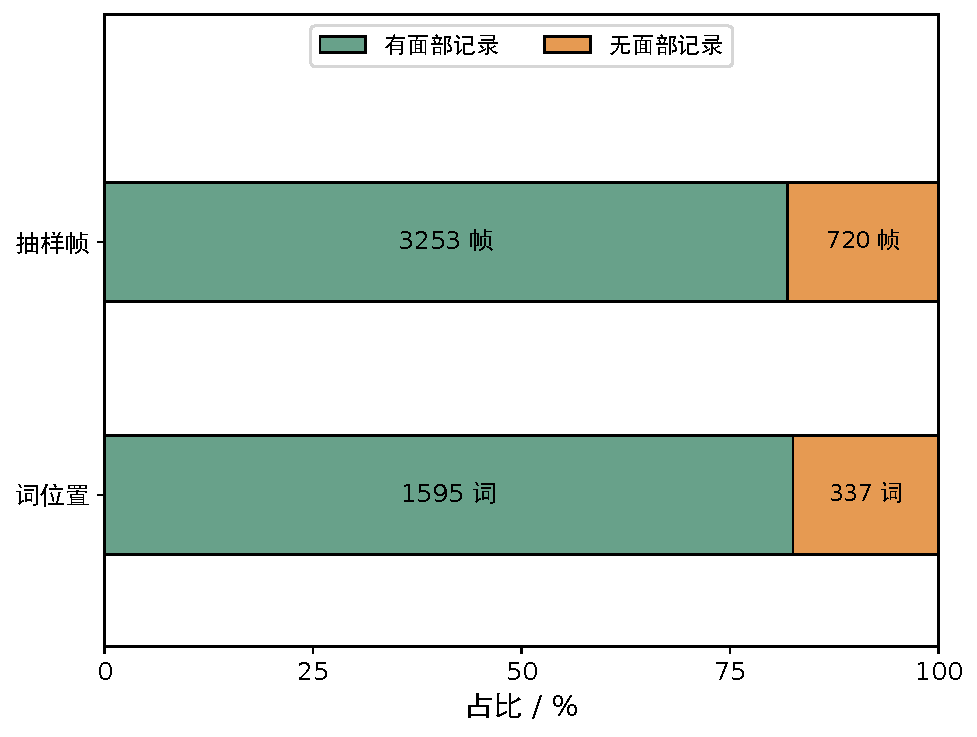
\includegraphics[width=\linewidth]{figures/fig_p1_visual_coverage.pdf}
        \caption{面部特征的帧级与词级覆盖}
        \label{fig:p1_visual_coverage}
    \end{minipage}\hfill
    \begin{minipage}[b]{.48\linewidth}
        \centering
        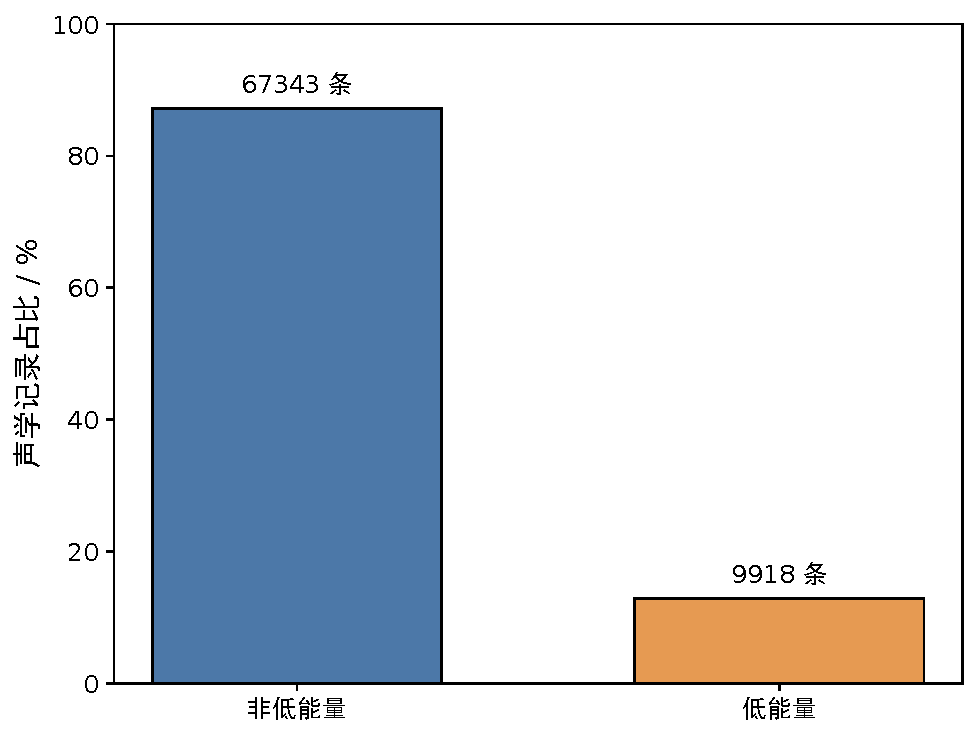
\includegraphics[width=\linewidth]{figures/fig_p1_audio_energy_share.pdf}
        \caption{声学记录的低能量占比}
        \label{fig:p1_audio_energy_share}
    \end{minipage}
\end{figure}

图~\ref{fig:p1_rms}与图~\ref{fig:p1_rms_zoom}以样本\nolinkurl{-iRBcNs9oI8$_$9}说明上述标记的时间分布。该样本333条RMS记录中有147条低于阈值；完整幅度图显示若干较强峰值，保持相同横轴的低幅值放大图则呈现峰值之间及片段末端的低能量区间。橙色虚线为阈值，橙点为低于阈值的记录。两图表明，声学输入状态随时间变化，采用逐记录标记能够保留整段平均统计无法呈现的局部差异。

\begin{figure}[H]
    \centering
    \begin{minipage}[b]{.48\linewidth}
        \centering
        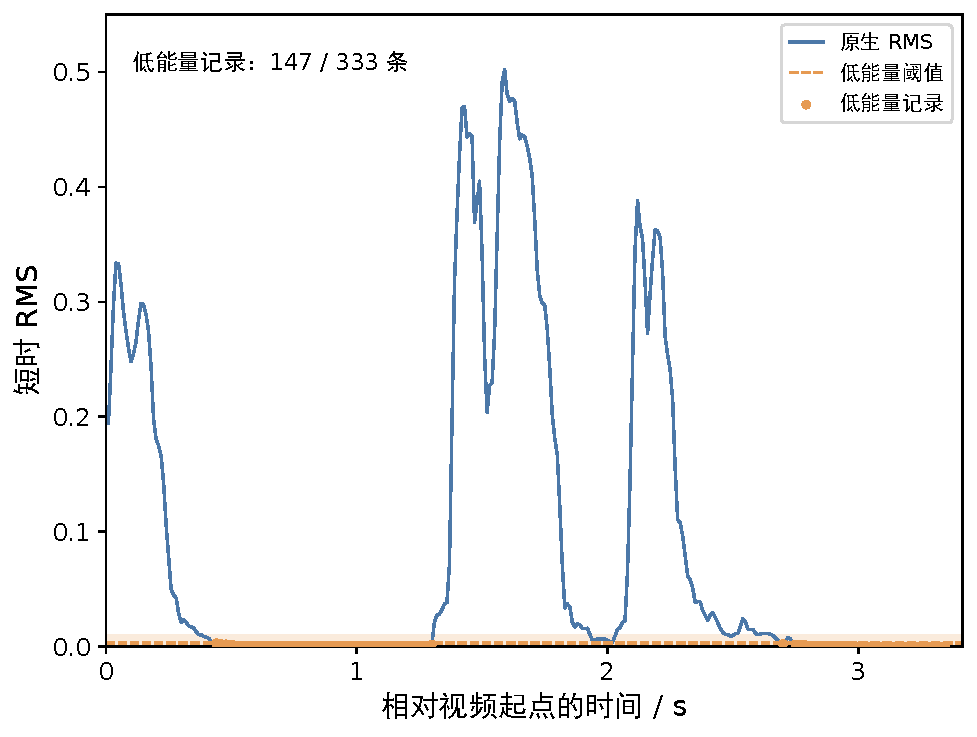
\includegraphics[width=\linewidth]{figures/fig_p1_rms.pdf}
        \caption{实例音频的短时RMS}
        \label{fig:p1_rms}
    \end{minipage}\hfill
    \begin{minipage}[b]{.48\linewidth}
        \centering
        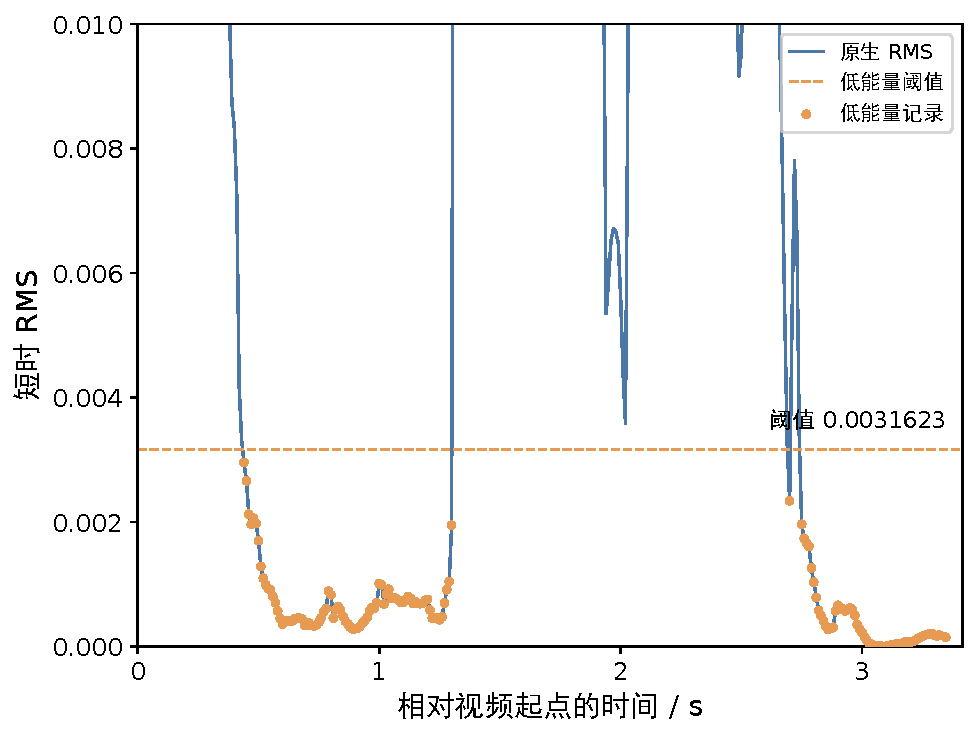
\includegraphics[width=\linewidth]{figures/fig_p1_rms_zoom.pdf}
        \caption{同一时间范围的低幅值放大}
        \label{fig:p1_rms_zoom}
    \end{minipage}
\end{figure}

另有两条样本的解码音频波形全为零，其声学特征各维均不随时间变化。结合视觉缺失与声学低能量结果可知，样本覆盖、模态观测和转写对应关系需要分别检查。本文保留全部样本及原始词位置，对视觉缺失采用零向量占位和无效标记，对低能量记录保留幅度状态；这种处理既维持了输入与输出的一一对应，也使异常位置能够被单独识别。在此基础上，下一步需要判断候选词时间区间是否得到实际音频的支持。

\subsubsection{时序对齐质量评估与人工审核}
\label{sec:p1_timing_quality}

前文的词级聚合以候选时间区间为依据，其可靠性直接影响哪些声学和视觉记录被分配到同一词位置。因此，时序组织的检查不能停留在矩阵行数一致，还需要评估给定转写与实际语音的匹配情况。本次CTC强制对齐为1932个词均生成候选区间，但满足字符路径约束只能说明算法获得了合法解，不能保证真实词界准确。本文据此设置局部词匹配与整段文本差异两个诊断层次，并用人工审核解释整段异常。

词级置信度取最优CTC路径中属于该词的文字字符帧概率的几何平均，不含空白符和词界符，用于描述模型对局部匹配的支持程度。片段级诊断词错误率（Word Error Rate，WER）则将无转写约束的贪心识别文本与规范化转写比较，以最少词编辑数除以参考词数，反映整段文本的差异。二者分别考察局部与整体：某些词即使得分较高，也可能处于整段内容不对应的片段中。由于两项指标来自同一声学模型，以下将其用于质量筛查，而不将其视为独立的词界准确性评价；WER包含插入操作，取值可以超过1。

图~\ref{fig:p1_ctc_confidence}与图~\ref{fig:p1_diagnostic_wer}显示，词级置信度与片段级WER均存在需要关注的异常区域。1932个词的置信度中位数为0.9585，1034个词不低于0.95，但仍有350个词低于0.1；100条片段的诊断WER均值为0.4689，其中21条超过0.8，9条超过1。图中的虚线和阴影分别标示对应阈值与关注区域。这些结果说明，整体较高的词级得分不足以支持无差别使用全部候选区间，需要进一步结合片段状态确定可用范围。

\begin{figure}[H]
    \centering
    \begin{minipage}[b]{.48\linewidth}
        \centering
        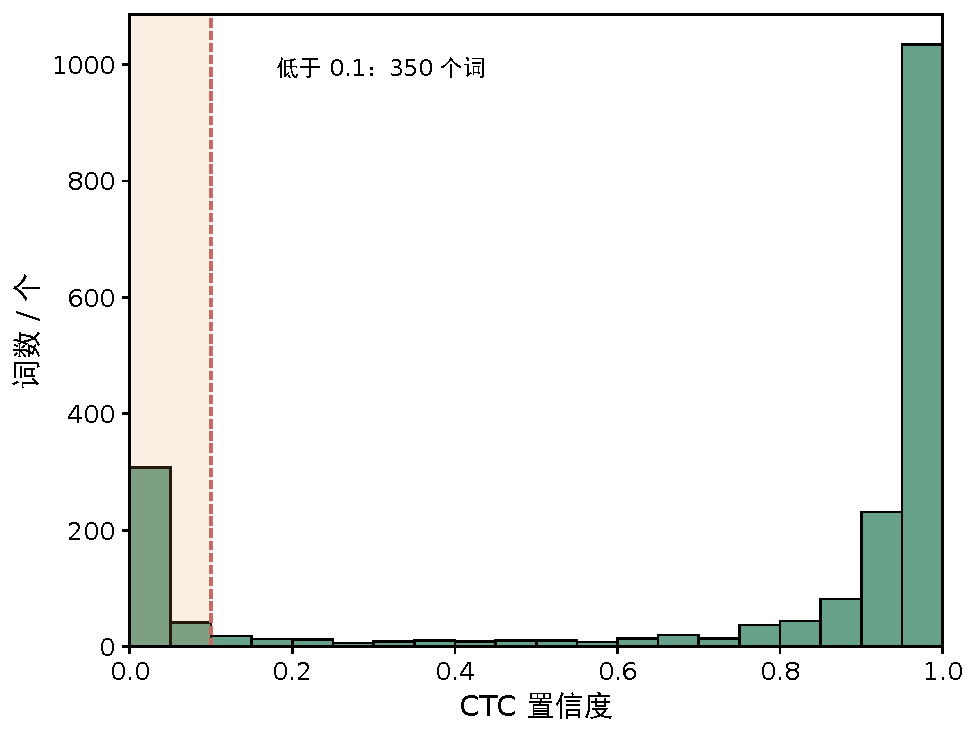
\includegraphics[width=\linewidth]{figures/fig_p1_ctc_confidence.pdf}
        \caption{词级CTC置信度分布}
        \label{fig:p1_ctc_confidence}
    \end{minipage}\hfill
    \begin{minipage}[b]{.48\linewidth}
        \centering
        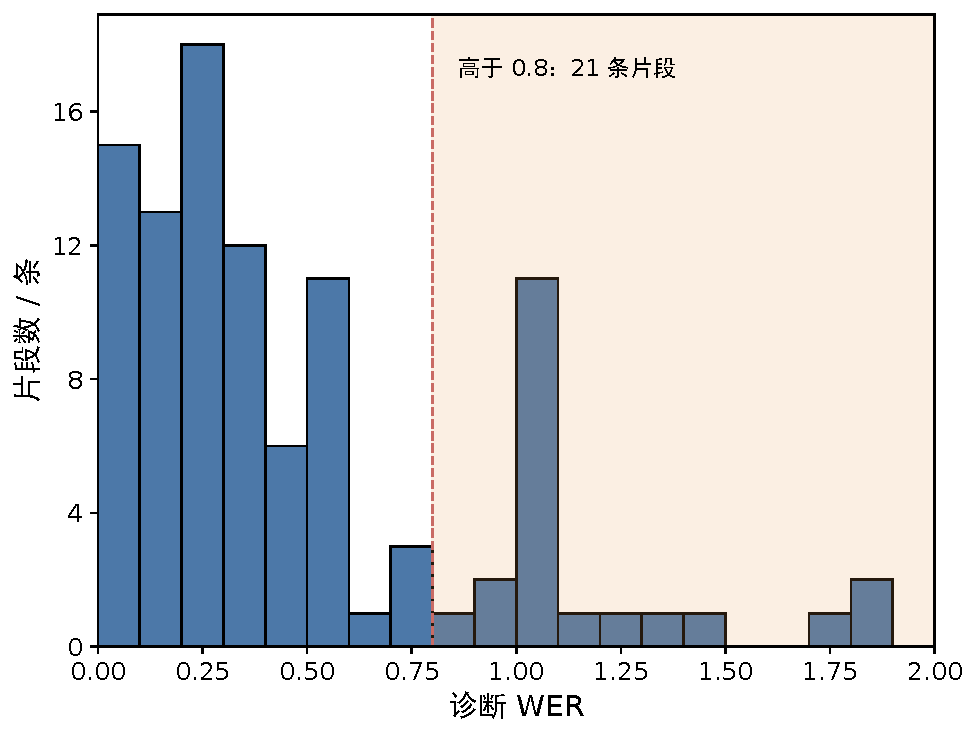
\includegraphics[width=\linewidth]{figures/fig_p1_diagnostic_wer.pdf}
        \caption{片段级诊断WER分布}
        \label{fig:p1_diagnostic_wer}
    \end{minipage}
\end{figure}

本文采用片段级与逐词两层筛选，将上述诊断落实为可随特征文件保存的质量标记。首先，平均词置信度低于0.2、置信度低于0.1的词超过一半、诊断WER大于0.8，或无法形成完整CTC路径的样本均列入整段复核，暂不采用其词级时间对应。其次，在其余样本中，仅将成功获得候选起止时间且置信度不低于0.1的词计为通过筛选。这些阈值作为保守检查条件，未利用情感标签或人工词界标注优化；筛选改变的是词级对应的使用标记，不删除样本、词位置或原始特征。

图~\ref{fig:p1_quality_flow}将两层筛选与模态观测检查串联起来。在100条样本中，19条的平均词置信度低于0.2，20条有超过一半的词置信度低于0.1，21条的诊断WER大于0.8，没有样本因无法形成完整CTC路径而被标记。这四项条件分别检查，每条样本只要满足其中任一项就进入整段复核；同一样本可能同时满足多项条件，因此各项数量不能直接相加。本次前两项标记的样本均已包含在WER大于0.8的21条样本中，去除重复计数后，需整段复核的仍为21条，共涉及317个词。其余79条样本包含1615个词，其中70个因置信度不足未通过逐词筛选，剩余1545个通过筛选，占全部词的79.97\%。这1545个词中，158个缺少有效面部记录，1387个同时满足对齐筛选和三模态可观测条件，占全部词的71.79\%。

\begin{figure}[H]
    \centering
    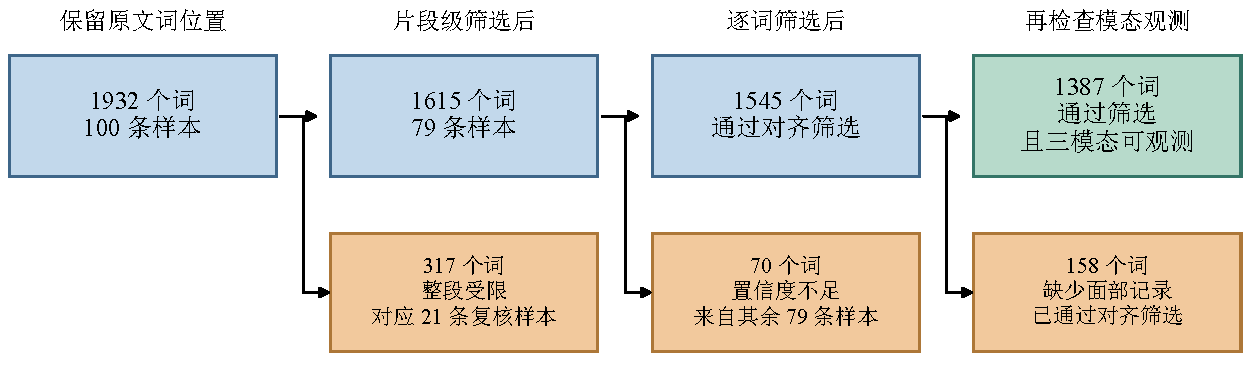
\includegraphics[width=\linewidth]{figures/fig_p1_quality_flow.pdf}
    \caption{从全部词位置到满足不同使用条件的词位置：各分支数量可逐项核对}
    \label{fig:p1_quality_flow}
\end{figure}

图中各分支均对应明确的使用条件，而非对原始数据的删减。317个整段受限词中包含37个局部置信度达到阈值的词，因而未通过筛选的387个词多于低置信度词的350个。另一方面，通过时间筛选但缺少面部记录的158个词仍保有文本与声学信息，只是不满足三模态同时可观测的条件。因此，后续读取词级输出时需要分别使用对齐质量标记与模态观测标记，区分“存在可计算记录”和“满足当前对齐筛选条件”这两种状态。

进一步将片段平均置信度阈值取0.1、0.2、0.3，诊断WER阈值取0.6、0.8、1.0，其余条件保持不变。在三种平均置信度阈值下，待复核样本数均随WER阈值变化依次为25、21、20条，表明当前数据的复核数量主要受WER条件影响。该检查反映筛选范围对阈值的敏感性，不能据此确定最优阈值或计算真实对齐准确率。

\label{sec:p1_window_analysis}
上述筛选回答了候选时间对应的使用范围，但尚未说明采用何种时间单元组织特征更便于保留信息。前文以词作为共同单位，是为了使文本语义单元与相应时段的视听记录保持明确联系。为考察统一时间切分可能带来的影响，本文在相同原生特征上构造0.2~s和0.5~s固定窗口作为补充对照，窗口均从零时刻开始，末窗截取至片段终点，并沿用有效时间交叠加权规则。该实验关注平均聚合对局部变化的保留程度，以及固定边界对词区间完整性的影响，为时间组织方式的合理性分析提供依据。

固定窗口对照包含聚合与重建两个步骤：首先分别聚合两种窗口内的原生特征，再根据时间交叠关系将窗口特征映回原生记录位置，以便与原序列比较。图~\ref{fig:p1_window_reconstruction}以响度展示重建结果，青蓝色线为原生记录，蓝线与橙线分别对应短窗和长窗。窗口平均削弱了原曲线的局部峰谷，较长窗口的平滑范围更大，说明统一时间汇总在压缩序列的同时会改变局部特征变化。这里的重建对象是特征序列，而非原始音频波形。

图~\ref{fig:p1_word_window_overlap}检查同一样本中的词区间是否被固定窗口切分。绿色线为\texttt{successful}的候选区间$[1.84247,2.40247]\,\mathrm{s}$，上、下两排分别为0.2~s和0.5~s窗口。该词分别与4个短窗和2个长窗交叠，在两种划分下均计为一个跨界词。第四个短窗的交叠仅约0.00247~s，图中以箭头注明；统计时将大于$10^{-8}\,\mathrm{s}$的交叠视为有效交叠。跨界指标只判断是否与至少两个窗口交叠，不区分交叠窗口数量及切分幅度。

上述图示采用样本\nolinkurl{-egA8-b7-3M$_$1}。其选取条件为未触发整段复核、面部观测帧占比不低于80\%，且时长最接近10~s。该样本实际时长10.266~s，包含20个词，其中18个通过对齐筛选。

\begin{figure}[H]
    \centering
    \begin{minipage}[b]{.48\linewidth}
        \centering
        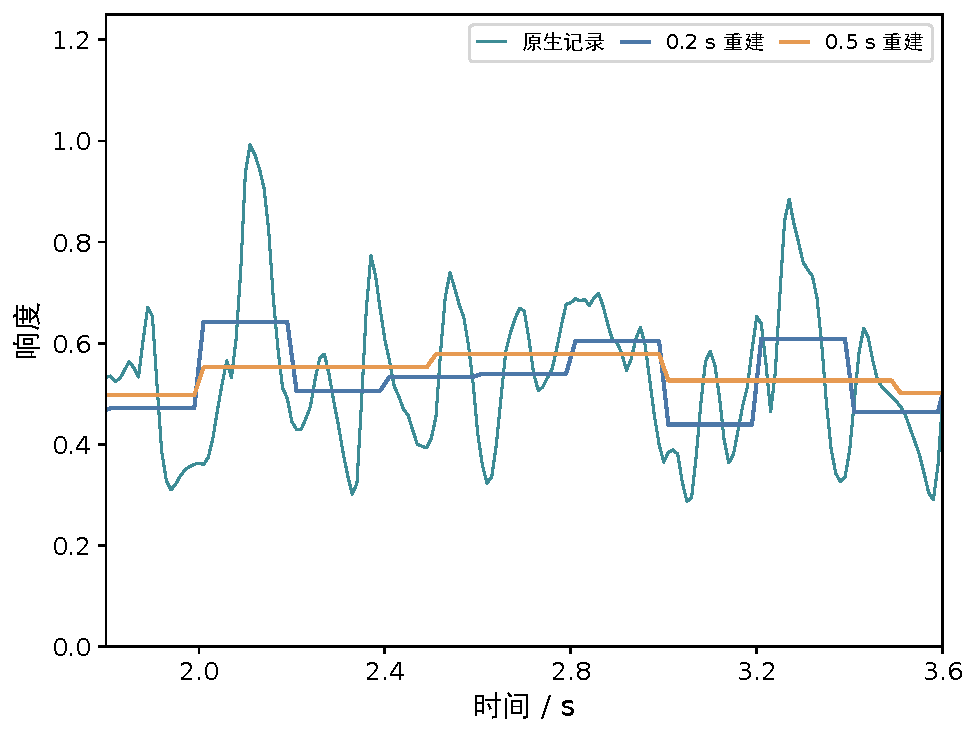
\includegraphics[width=\linewidth]{figures/fig_p1_window_reconstruction.pdf}
        \caption{响度的固定窗口聚合与重建}
        \label{fig:p1_window_reconstruction}
    \end{minipage}\hfill
    \begin{minipage}[b]{.48\linewidth}
        \centering
        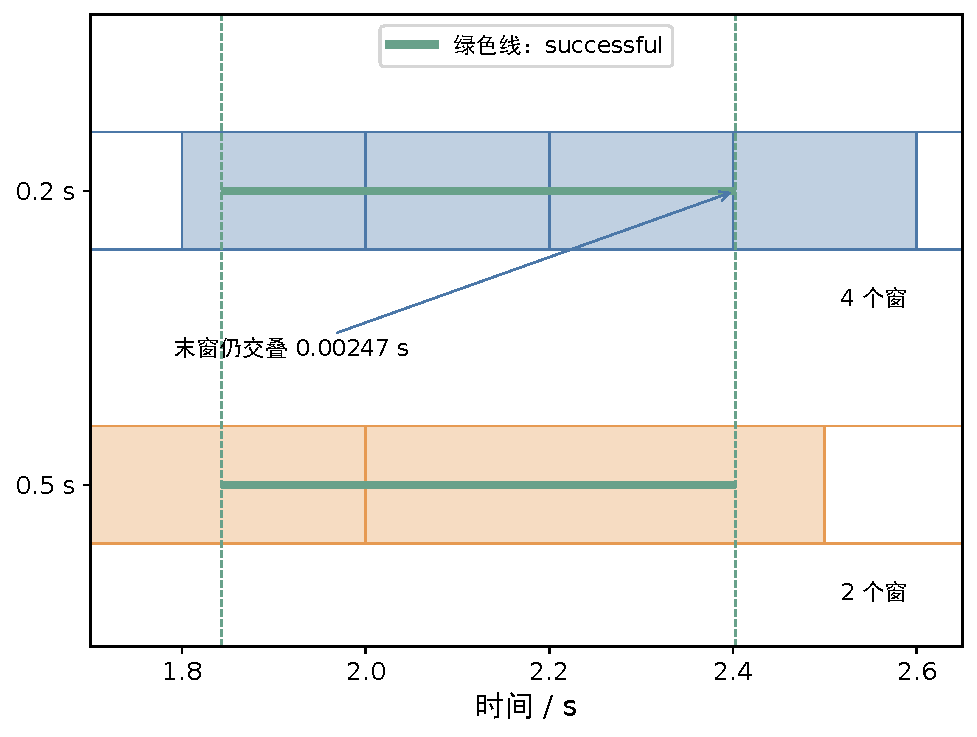
\includegraphics[width=\linewidth]{figures/fig_p1_word_window_overlap.pdf}
        \caption{候选词区间与固定窗口交叠}
        \label{fig:p1_word_window_overlap}
    \end{minipage}
\end{figure}

为判断上述现象是否仅出现在个别片段，本文对全量样本分别计算标准化重建均方误差与词跨界比例。重建误差将重建特征与原生特征之差按各维原生标准差归一化，再对有效记录和维度的平方误差取平均，数值越低表示越接近原生特征；仅纳入标准差大于$10^{-6}$的维度，有记录但全部维度恒定时记0，无有效记录时不计入模态均值。词跨界比例则在每条样本通过对齐筛选的词中，统计与至少两个窗口交叠的词所占比例，数值越高表示被切分的词越多。两类指标均先在样本内计算，再对相应有效样本等权平均，以区分特征变化的保留程度和词区间的完整性。

图~\ref{fig:p1_audio_window_error}至图~\ref{fig:p1_word_crossing_ratio}汇总全量对照。声学与视觉重建误差图中的短窗箱体整体低于长窗箱体，声学平均重建误差由0.7467降至0.5449，视觉由0.4373降至0.2357，相对降幅分别为27.02\%和46.10\%。图~\ref{fig:p1_word_crossing_ratio}则呈相反方向，平均词跨界比例由39.50\%升至71.33\%，增加31.83个百分点。三幅图分别基于100条声学样本、87条具有有效面部记录的样本和79条未触发整段复核的样本。图中菱形标出均值，箱内横线标出中位数，箱体覆盖第25至第75百分位数，须线延伸至1.5倍四分位距内的最远观测；箱外圆点仍参与统计。

\begin{figure}[H]
    \centering
    \begin{minipage}[b]{.32\linewidth}
        \centering
        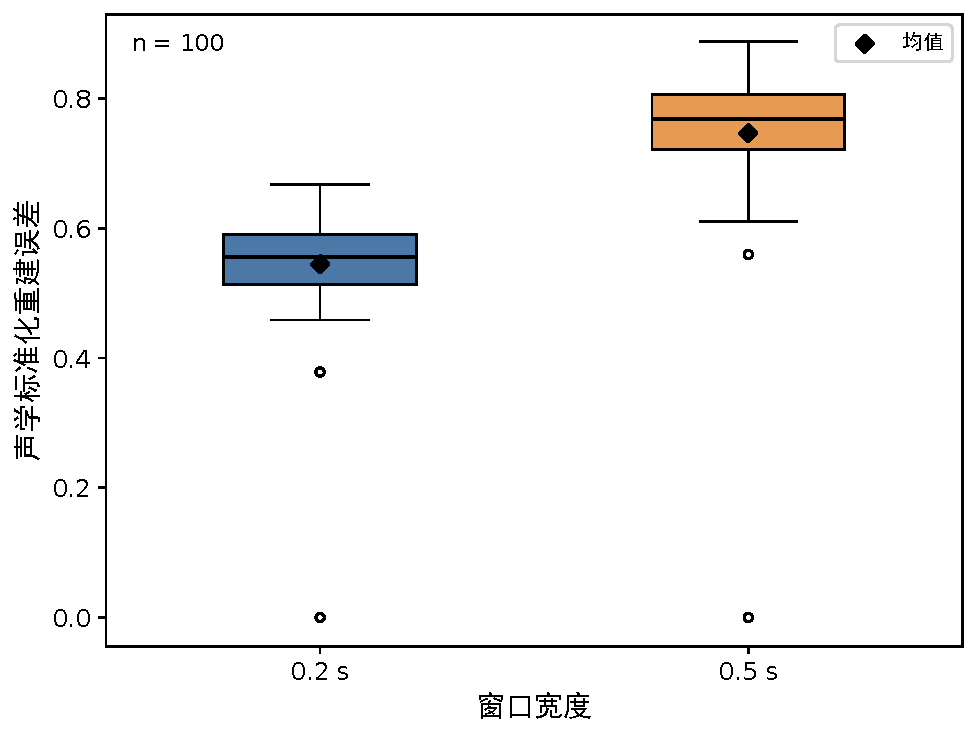
\includegraphics[width=\linewidth]{figures/fig_p1_audio_window_error.pdf}
        \caption{声学重建误差对照}
        \label{fig:p1_audio_window_error}
    \end{minipage}\hfill
    \begin{minipage}[b]{.32\linewidth}
        \centering
        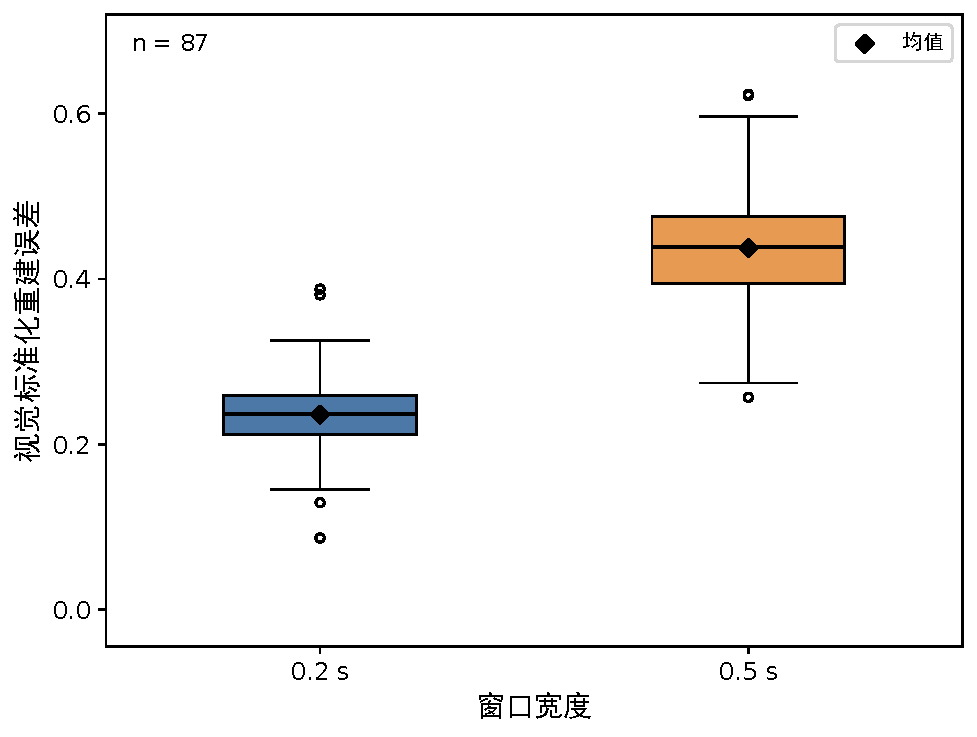
\includegraphics[width=\linewidth]{figures/fig_p1_vision_window_error.pdf}
        \caption{视觉重建误差对照}
        \label{fig:p1_vision_window_error}
    \end{minipage}\hfill
    \begin{minipage}[b]{.32\linewidth}
        \centering
        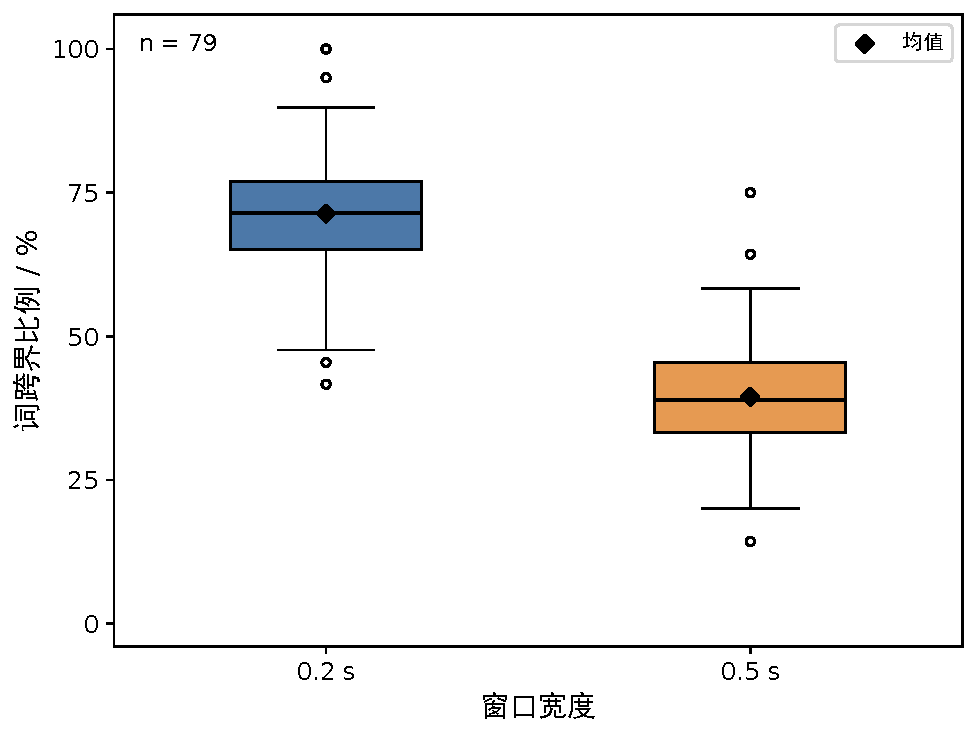
\includegraphics[width=\linewidth]{figures/fig_p1_word_crossing_ratio.pdf}
        \caption{词跨界比例对照}
        \label{fig:p1_word_crossing_ratio}
    \end{minipage}
\end{figure}

逐样本比较进一步表明，98条样本的短窗声学误差更低，另2条相同；87条样本的短窗视觉误差均更低；77条样本的短窗词跨界比例更高，另2条相同。两条声学误差相同的样本即前述全零音频样本，其特征不随时间变化，两种窗口的误差均按规则记0。将这两条样本单独列出后，其余98条样本的短窗、长窗平均声学误差分别为0.5560和0.7619，差异方向保持一致。两种窗口的200条逐样本指标详见问题一提交附件中的\nolinkurl{step1/validation/audited_window_comparison.csv}，剔除恒定声学样本后的统计及相对变化量见同目录下的\nolinkurl{analysis_statistics.json}。

上述对照表明，在本次数据与窗口设置下，缩短窗口有利于保留原生特征的局部变化，却同时增加了词区间被固定边界切分的比例。因此，仅通过调整统一窗口宽度，仍需在这两个目标之间进行权衡。这一现象说明，以原文词为组织单位、再根据候选词区间聚合视听记录具有明确的任务动机：它使词级表示直接对应一个文本单元，并保留参与聚合的原生记录供回溯使用。不过，本实验未直接比较词级表示的重建误差，也未引入人工词界或情感预测任务，故不能据此断言词级表示在上述指标上优于固定窗口；其时间对应质量仍取决于候选词界及观测状态。

时间划分对照解释了聚合粒度的影响，而21条整段受限样本还涉及更基本的前提：给定英文转写是否具有相应的语音依据。若输入内容不对应，即使强制对齐能够生成完整路径，其候选词界也缺少真实发音支撑。为区分输入异常与一般的词界定位偏差，本文进一步对照实际音频和给定转写进行人工审核，按主要问题划分为表~\ref{tab:p1_manual_review}所列五类。各类互不重叠，共涉及317个原文词。

\begin{table}[H]
    \centering\small
    \caption{21条复核样本的人工审核结果}
    \label{tab:p1_manual_review}
    \setlength{\tabcolsep}{6pt}
    \renewcommand{\arraystretch}{1.12}
    \ifdefined\pOneCompactTableBox\else\newsavebox{\pOneCompactTableBox}\fi
    \begin{lrbox}{\pOneCompactTableBox}
    \begin{tabular}{lcc>{\raggedright\arraybackslash}p{18em}}
        \toprule
        审核发现 & 样本数 & 原文词数 & 主要表现\\
        \midrule
        音轨与文本不对应 & 11 & 120 & 实际语音内容与给定转写不对应\\
        无对应朗读 & 5 & 64 & 未听到对应朗读，其中1条为音乐\\
        非英语语音 & 3 & 93 & 实际语音并非英语\\
        分段内容不对应 & 1 & 18 & 前半段无朗读，后半段语音与转写不对应\\
        音频卡顿、局部对应 & 1 & 22 & 音频存在卡顿，部分词语与文本一致，但未形成完整对应\\
        \midrule
        合计 & 21 & 317 & \\
        \bottomrule
    \end{tabular}
    \end{lrbox}
    \usebox{\pOneCompactTableBox}
\end{table}

审核发现，音轨与文本不对应、缺少对应朗读等情况使给定转写缺少相应的语音依据；非英语语音则与所用英语声学模型及英文对齐目标不匹配。其中，3条非英语样本均来自视频\nolinkurl{-yRb-Jum7EQ}，两条全零音频样本归入“无对应朗读”。这些异常具有不同来源，不能统一解释为词界定位偏差。

样本\nolinkurl{-HwX2H8Z4hY$_$9}还说明了片段级检查的必要性。其平均词置信度为0.7238，仅9.09\%的词低于0.1，但诊断WER达到0.8636。人工审核发现音频存在卡顿，部分词语与转写一致，却没有形成完整逐词对应，说明局部得分较高不足以确认整段对应关系。

依据审核结果，本文维持这21条样本整体词级对应受限的标记，同时保留其原文、标签、原生特征与候选时间记录。该处理遵循题目关于保留原始样本并说明异常处理规则的要求，使内容对应异常能够被追溯，而不会通过修改转写或删除样本被隐去。由于本次审核未重建人工词界，不恢复局部词的对齐标记，前述筛选数量保持不变。审核范围仅为自动筛出的21条样本，不能据此认定其余79条均无异常，也不能计算全量词界准确率。逐样本的问题分类与审核说明详见问题一提交附件中的\nolinkurl{step1/results/}\textnormal{人工审核\_21条样本.csv}。

\subsubsection{典型样本的跨模态时序对齐验证}
\label{sec:p1_verification_examples}

全量统计明确了输出的使用范围，典型样本则进一步检验具体记录能否回溯到原始素材。本文继续采用样本\nolinkurl{-egA8-b7-3M$_$1}，展示文本片段、语音时段、视频帧及三类特征之间的对应。该样本给定转写包含“I started a successful Legal Nurse Consulting Business in 1989.”，图~\ref{fig:p1_multimodal_result}选取其中1.80--3.60~s的局部时段，自上而下排列实际画面、候选词区间、响度及面部系数。通过共同时间轴，可以从一个原文词定位其对应的声学记录与视频帧；其中浅绿底突出\texttt{successful}的候选区间，其内约2.11~s处出现响度峰值。图片按标注时刻定位，图片宽度不代表持续时间，面部曲线连线仅辅助观察。

\begin{figure}[H]
    \centering
    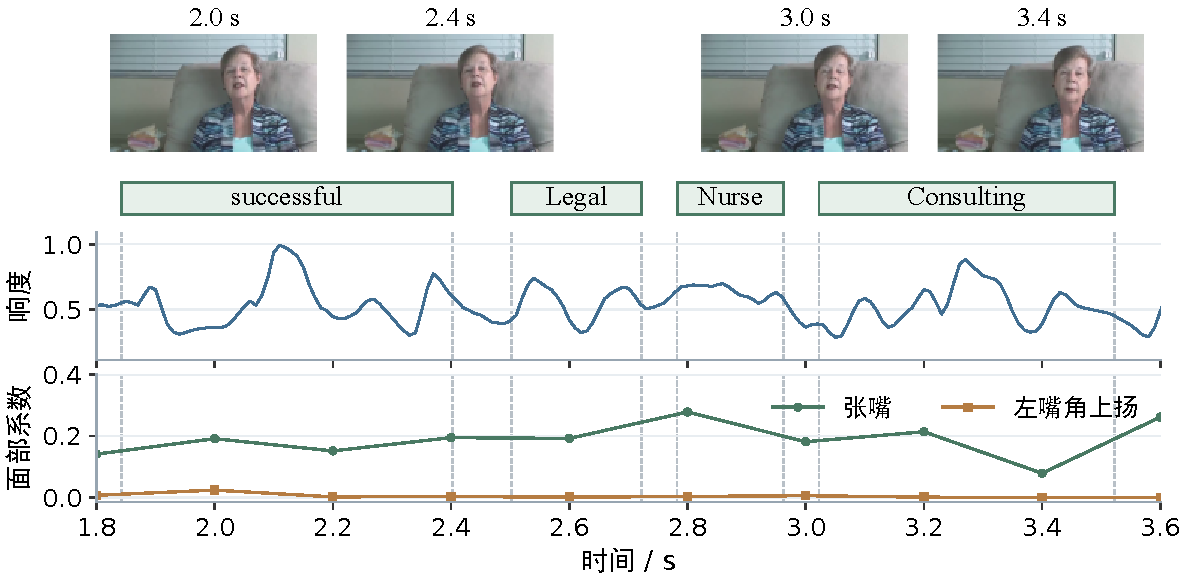
\includegraphics[width=\linewidth]{figures/fig_p1_multimodal_timeline.pdf}
    \caption{词级映射的回溯示例：从候选词区间定位同一时段的声音与画面}
    \label{fig:p1_multimodal_result}
\end{figure}

表~\ref{tab:p1_mapping_records}列出部分映射记录。词\textit{successful}的候选区间为$[1.8425,2.4025]\,\mathrm{s}$，文本表示由子词索引3对应的隐藏向量获得，声学表示由183--240号共58条原生记录聚合，视觉表示由1.8、2.0、2.2、2.4~s四帧聚合。由此，该词的768维文本、25维声学与52维视觉向量均可回溯到各自来源。索引从0开始；声学索引指特征记录而非波形采样点，视觉帧依据时间支持区间参与聚合，因此帧中心可以位于词区间之外，边界帧的权重由实际交叠时长决定。该样本全部词的映射明细见问题一提交附件中的\nolinkurl{step1/results/typical_feature_mapping.csv}；完整向量和聚合权重保存在该样本目录的\nolinkurl{features.npz}中。

\begin{table}[H]
    \centering\small
    \caption{典型样本的部分词级映射记录}
    \label{tab:p1_mapping_records}
    \setlength{\tabcolsep}{6pt}
    \renewcommand{\arraystretch}{1.12}
    \ifdefined\pOneCompactTableBox\else\newsavebox{\pOneCompactTableBox}\fi
    \begin{lrbox}{\pOneCompactTableBox}
    \begin{tabular}{lcccc}
        \toprule
        原文词 & 子词索引 & 候选区间/s & 声学记录索引 & 视觉帧时刻/s\\
        \midrule
        started & 1 & $[1.2825,1.6425]$ & 127--164 & 1.2, 1.4, 1.6\\
        successful & 3 & $[1.8425,2.4025]$ & 183--240 & 1.8, 2.0, 2.2, 2.4\\
        Consulting & 6 & $[3.0225,3.5225]$ & 301--352 & 3.0, 3.2, 3.4, 3.6\\
        \bottomrule
    \end{tabular}
    \end{lrbox}
    \usebox{\pOneCompactTableBox}
\par\smallskip
\parbox{\wd\pOneCompactTableBox}{\footnotesize 注：索引从0开始；声学索引指具有正聚合权重的原生特征记录，不是波形采样点。视觉帧按其时间支持区间与候选词区间的交叠关系参与聚合，帧中心不必位于词区间内部。}
\end{table}

典型样本图与映射表共同展示了从原文词到模型子词、声学记录和视频帧的可追溯链条，使前文的聚合规则能够在具体输出上核验。进一步对全部100条样本独立复算交叠权重、视听聚合值和CTC置信度，重新计算诊断WER，并解码音视频核对时间记录与低能量标记，结果均在既定数值容差内与保存记录一致。这一检查验证了实现与既定计算规则的一致性；真实词界精度仍需人工时间标注评价。典型样本中的\texttt{in}和\texttt{1989}也继续保留置信度不足的标记，说明实例展示与质量筛选采用相同标准，没有因为选作典型样本而放宽使用条件。全量路径与聚合核验记录见问题一提交附件中的\nolinkurl{step1/results/verification.json}，媒体解码及各项统计的独立复算记录见\nolinkurl{step1/validation/data_audit.json}。

\subsubsection{三模态特征文件说明与100条样本结果汇总}
\label{sec:p1_delivery}

以上统计与典型样本展示说明了输出的覆盖范围、质量状态和回溯方式。为进一步满足题目对自生成特征文件规范及全部100条样本结果汇总的要求，本文采用“统一模态规格＋逐样本明细”的组织方式：表~\ref{tab:p1_feature_specification}列出每条样本共有的模态类型、特征维数、矩阵形状与对齐粒度，表~\ref{tab:p1_all_samples}列出全部样本的编号、原始媒体时长及有效位置统计。两表结合，可确定任一样本三种模态的输出规格及使用范围；具体高维数值由相应样本目录中的特征文件提供。

\begin{table}[H]
    \centering\small
    \caption{三种模态的词级特征规格}
    \label{tab:p1_feature_specification}
    \setlength{\tabcolsep}{6pt}
    \renewcommand{\arraystretch}{1.12}
    \ifdefined\pOneCompactTableBox\else\newsavebox{\pOneCompactTableBox}\fi
    \begin{lrbox}{\pOneCompactTableBox}
    \begin{tabular}{lccc}
        \toprule
        模态 & 特征维数 & 样本矩阵形状 & 对齐粒度\\
        \midrule
        文本 & 768 & $L\times768$ & 原文词\\
        声学 & 25 & $L\times25$ & 原文词\\
        视觉（面部） & 52 & $L\times52$ & 原文词\\
        \bottomrule
    \end{tabular}
    \end{lrbox}
    \usebox{\pOneCompactTableBox}
\par\smallskip
\parbox{\wd\pOneCompactTableBox}{\footnotesize 注：$L$为对应样本的原文词数。各样本按实际词数存储，填充数与截断词数均为0；视觉模态不可观测的词位置采用零向量占位，并附无效标记。}
\end{table}

在时序组织上，每条样本按实际原文词数$L$保存变长序列，不进行统一长度填充或截断。$L$表示保留的词位置总数，模态观测有效位置数与通过对齐筛选的位置数另由掩码统计；这些位置不必连续，因此不能仅保存一个长度数值而省略逐位置标记。视觉无效位置的零向量用于在原词位置上占位，含义不同于在序列末尾追加的长度填充。

全量表中，“原文词数”对应三个矩阵的行数，“视觉可观测词数”统计能聚合有效面部记录的位置，“通过对齐筛选词数”依据前述两层筛选条件，最后一列为通过筛选且三种模态均可观测的词数。由于文本与声学在全部词位置均有可计算记录，最后一列等于对齐筛选与视觉可观测两个条件的交集。片段时长与音频时长均按前文的实际解码口径记录，用于定位原始媒体的时间范围，不将其解释为有效发声或面部可观测的累计时长。

例如，样本-s9qJ7ATP7w\$\_\$7共有28个词，其中14个视觉可观测，24个通过对齐筛选，同时满足两项条件的有12个。交集数量不能取前两项数量的较小值代替。

按上述口径，32条样本的全部词通过筛选且三种模态均可观测，46条样本仅部分词满足两项条件，1条样本的全部词通过对齐筛选但视觉模态不可观测，另21条样本经人工审核后整体词级对应仍受限。全量表按这四类依次排列，已审核的21条样本统一归入最后一类，各组互不重叠。与表~\ref{tab:p1_all_samples}对应的电子清单见问题一提交附件中的\nolinkurl{step1/results/}\textnormal{全部样本特征交付清单.csv}，可按样本编号检索和核对各项统计。

\begingroup
\small
\setlength{\tabcolsep}{6pt}
\renewcommand{\arraystretch}{1.12}
\setlength{\LTleft}{\fill}
\setlength{\LTright}{\fill}
\begin{longtable}{lrrrrrr}
\caption{附件1全部样本的特征输出与有效位置统计}\label{tab:p1_all_samples}\\
\toprule
样本编号 & \shortstack{片段\\时长/s} & \shortstack{音频\\时长/s} & \shortstack{原文\\词数} & \shortstack{视觉可观测\\词数} & \shortstack{通过对齐\\筛选词数} & \shortstack{其中三种模态\\都可观测\\词数}\\
\midrule
\endfirsthead
\multicolumn{7}{c}{表~\thetable\quad 特征输出与有效位置统计（续）}\\
\toprule
样本编号 & \shortstack{片段\\时长/s} & \shortstack{音频\\时长/s} & \shortstack{原文\\词数} & \shortstack{视觉可观测\\词数} & \shortstack{通过对齐\\筛选词数} & \shortstack{其中三种模态\\都可观测\\词数}\\
\midrule
\endhead
\midrule
\multicolumn{7}{r}{续下页}\\
\endfoot
\bottomrule
\endlastfoot
\multicolumn{7}{l}{\textbf{1. 全部词通过筛选且三种模态都可观测（32条）}}\\*
\nolinkurl{-3g5yACwYnA$_$3} & 14.389 & 14.328 & 29 & 29 & 29 & 29\\
\nolinkurl{-3nNcZdcdvU$_$5} & 7.868 & 7.789 & 18 & 18 & 18 & 18\\
\nolinkurl{-6rXp3zJ3kc$_$8} & 12.805 & 12.738 & 34 & 34 & 34 & 34\\
\nolinkurl{-I_e4mIh0yE$_$1} & 7.622 & 7.444 & 18 & 18 & 18 & 18\\
\nolinkurl{-I_e4mIh0yE$_$3} & 9.163 & 8.994 & 22 & 22 & 22 & 22\\
\nolinkurl{-MeTTeMJBNc$_$0} & 9.333 & 9.218 & 21 & 21 & 21 & 21\\
\nolinkurl{-MeTTeMJBNc$_$13} & 5.430 & 5.255 & 14 & 14 & 14 & 14\\
\nolinkurl{-RfYyzHpjk4$_$11} & 5.239 & 5.075 & 17 & 17 & 17 & 17\\
\nolinkurl{-RfYyzHpjk4$_$8} & 4.589 & 4.532 & 17 & 17 & 17 & 17\\
\nolinkurl{-UUCSKoHeMA$_$0} & 7.867 & 7.732 & 18 & 18 & 18 & 18\\
\nolinkurl{-UacrmKiTn4$_$10} & 7.362 & 7.242 & 18 & 18 & 18 & 18\\
\nolinkurl{-UacrmKiTn4$_$4} & 4.741 & 4.682 & 14 & 14 & 14 & 14\\
\nolinkurl{-aNfi7CP8vM$_$7} & 8.695 & 8.538 & 18 & 18 & 18 & 18\\
\nolinkurl{-aqamKhZ1Ec$_$0} & 11.000 & 10.890 & 14 & 14 & 14 & 14\\
\nolinkurl{-dxfTGcXJoc$_$1} & 16.161 & 16.018 & 37 & 37 & 37 & 37\\
\nolinkurl{-egA8-b7-3M$_$16} & 5.538 & 5.483 & 11 & 11 & 11 & 11\\
\nolinkurl{-egA8-b7-3M$_$17} & 7.271 & 7.095 & 16 & 16 & 16 & 16\\
\nolinkurl{-egA8-b7-3M$_$18} & 8.386 & 8.266 & 22 & 22 & 22 & 22\\
\nolinkurl{-egA8-b7-3M$_$20} & 6.645 & 6.474 & 20 & 20 & 20 & 20\\
\nolinkurl{-egA8-b7-3M$_$26} & 6.031 & 5.921 & 15 & 15 & 15 & 15\\
\nolinkurl{-egA8-b7-3M$_$6} & 6.265 & 6.183 & 12 & 12 & 12 & 12\\
\nolinkurl{-egA8-b7-3M$_$9} & 5.090 & 4.936 & 10 & 10 & 10 & 10\\
\nolinkurl{-mqbVkbCndg$_$0} & 6.500 & 6.386 & 14 & 14 & 14 & 14\\
\nolinkurl{-s9qJ7ATP7w$_$6} & 2.475 & 2.315 & 5 & 5 & 5 & 5\\
\nolinkurl{-s9qJ7ATP7w$_$8} & 3.295 & 3.184 & 12 & 12 & 12 & 12\\
\nolinkurl{-t217m2on-s$_$7} & 17.183 & 17.026 & 45 & 45 & 45 & 45\\
\nolinkurl{-tPCytz4rww$_$10} & 4.789 & 4.679 & 12 & 12 & 12 & 12\\
\nolinkurl{-tPCytz4rww$_$11} & 5.467 & 5.379 & 17 & 17 & 17 & 17\\
\nolinkurl{-tPCytz4rww$_$18} & 6.645 & 6.569 & 16 & 16 & 16 & 16\\
\nolinkurl{-uywlfIYOS8$_$4} & 6.045 & 5.881 & 18 & 18 & 18 & 18\\
\nolinkurl{-wny0OAz3g8$_$0} & 3.333 & 3.274 & 9 & 9 & 9 & 9\\
\nolinkurl{-wny0OAz3g8$_$2} & 6.687 & 6.523 & 23 & 23 & 23 & 23\\
\addlinespace[0.5em]
\multicolumn{7}{l}{\textbf{2. 部分词通过筛选且三种模态都可观测（46条）}}\\*
\nolinkurl{-3g5yACwYnA$_$13} & 5.514 & 5.399 & 15 & 15 & 14 & 14\\
\nolinkurl{-3g5yACwYnA$_$2} & 9.394 & 9.231 & 14 & 14 & 13 & 13\\
\nolinkurl{-3g5yACwYnA$_$9} & 8.817 & 8.696 & 23 & 23 & 21 & 21\\
\nolinkurl{-571d8cVauQ$_$0} & 5.167 & 4.992 & 12 & 12 & 10 & 10\\
\nolinkurl{-571d8cVauQ$_$5} & 15.273 & 15.115 & 43 & 43 & 42 & 42\\
\nolinkurl{-9y-fZ3swSY$_$0} & 6.900 & 6.757 & 22 & 22 & 19 & 19\\
\nolinkurl{-9y-fZ3swSY$_$4} & 2.821 & 2.665 & 9 & 9 & 6 & 6\\
\nolinkurl{-9y-fZ3swSY$_$8} & 4.989 & 4.917 & 12 & 3 & 11 & 2\\
\nolinkurl{-AUZQgSxyPQ$_$2} & 22.511 & 22.405 & 41 & 41 & 39 & 39\\
\nolinkurl{-HeZS2-Prhc$_$2} & 8.262 & 8.151 & 16 & 16 & 15 & 15\\
\nolinkurl{-HwX2H8Z4hY$_$2} & 3.982 & 3.916 & 7 & 1 & 4 & 1\\
\nolinkurl{-HwX2H8Z4hY$_$5} & 5.653 & 5.544 & 9 & 2 & 8 & 2\\
\nolinkurl{-HwX2H8Z4hY$_$6} & 3.358 & 3.256 & 7 & 5 & 6 & 5\\
\nolinkurl{-MeTTeMJBNc$_$7} & 10.517 & 10.411 & 31 & 31 & 29 & 29\\
\nolinkurl{-RfYyzHpjk4$_$2} & 5.516 & 5.392 & 25 & 24 & 21 & 21\\
\nolinkurl{-THoVjtIkeU$_$12} & 14.896 & 14.806 & 39 & 39 & 38 & 38\\
\nolinkurl{-THoVjtIkeU$_$2} & 4.292 & 4.231 & 10 & 10 & 9 & 9\\
\nolinkurl{-THoVjtIkeU$_$6} & 8.097 & 7.983 & 30 & 30 & 27 & 27\\
\nolinkurl{-UuX1xuaiiE$_$0} & 3.700 & 3.576 & 9 & 6 & 8 & 5\\
\nolinkurl{-UuX1xuaiiE$_$1} & 10.350 & 10.268 & 27 & 1 & 27 & 1\\
\nolinkurl{-UuX1xuaiiE$_$3} & 4.130 & 4.038 & 9 & 9 & 8 & 8\\
\nolinkurl{-UuX1xuaiiE$_$6} & 8.114 & 7.944 & 22 & 22 & 20 & 20\\
\nolinkurl{-a55Q6RWvTA$_$3} & 22.154 & 22.083 & 65 & 60 & 63 & 58\\
\nolinkurl{-dxfTGcXJoc$_$0} & 20.533 & 20.410 & 40 & 33 & 39 & 32\\
\nolinkurl{-dxfTGcXJoc$_$2} & 16.698 & 16.633 & 34 & 34 & 33 & 33\\
\nolinkurl{-dxfTGcXJoc$_$6} & 12.735 & 12.628 & 28 & 28 & 27 & 27\\
\nolinkurl{-egA8-b7-3M$_$1} & 10.266 & 10.156 & 20 & 20 & 18 & 18\\
\nolinkurl{-egA8-b7-3M$_$13} & 4.184 & 4.024 & 11 & 11 & 10 & 10\\
\nolinkurl{-lzEya4AM_4$_$5} & 7.675 & 7.570 & 19 & 19 & 18 & 18\\
\nolinkurl{-lzEya4AM_4$_$6} & 14.792 & 14.740 & 43 & 43 & 42 & 42\\
\nolinkurl{-qDkUB0GgYY$_$6} & 4.678 & 4.615 & 16 & 16 & 12 & 12\\
\nolinkurl{-s9qJ7ATP7w$_$0} & 6.867 & 6.711 & 24 & 24 & 23 & 23\\
\nolinkurl{-s9qJ7ATP7w$_$1} & 4.792 & 4.644 & 11 & 11 & 10 & 10\\
\nolinkurl{-s9qJ7ATP7w$_$4} & 4.427 & 4.247 & 9 & 6 & 8 & 5\\
\nolinkurl{-s9qJ7ATP7w$_$5} & 8.561 & 8.398 & 19 & 19 & 18 & 18\\
\nolinkurl{-s9qJ7ATP7w$_$7} & 6.966 & 6.839 & 28 & 14 & 24 & 12\\
\nolinkurl{-t217m2on-s$_$2} & 5.686 & 5.630 & 12 & 12 & 11 & 11\\
\nolinkurl{-tANM6ETl_M$_$3} & 6.758 & 6.604 & 22 & 22 & 21 & 21\\
\nolinkurl{-tPCytz4rww$_$12} & 11.864 & 11.736 & 26 & 26 & 24 & 24\\
\nolinkurl{-tPCytz4rww$_$16} & 7.206 & 7.139 & 16 & 16 & 14 & 14\\
\nolinkurl{-vxjVxOeScU$_$4} & 9.127 & 9.037 & 21 & 21 & 18 & 18\\
\nolinkurl{-wMB_hJL-3o$_$7} & 6.044 & 5.976 & 22 & 22 & 21 & 21\\
\nolinkurl{-wny0OAz3g8$_$3} & 6.146 & 6.100 & 20 & 1 & 20 & 1\\
\nolinkurl{-wny0OAz3g8$_$5} & 6.912 & 6.741 & 20 & 1 & 20 & 1\\
\nolinkurl{-wny0OAz3g8$_$7} & 8.068 & 7.910 & 29 & 6 & 29 & 6\\
\nolinkurl{-wny0OAz3g8$_$9} & 6.213 & 6.043 & 20 & 20 & 19 & 19\\
\addlinespace[0.5em]
\multicolumn{7}{l}{\textbf{3. 全部词通过对齐筛选，但视觉模态不可观测（1条）}}\\*
\nolinkurl{-wny0OAz3g8$_$1} & 6.844 & 6.777 & 22 & 0 & 22 & 0\\
\addlinespace[0.5em]
\multicolumn{7}{l}{\textbf{4. 整段对齐受限（已完成人工审核）（21条）}}\\*
\nolinkurl{-HwX2H8Z4hY$_$9} & 7.734 & 7.636 & 22 & 0 & 0 & 0\\
\nolinkurl{-NFrJFQijFE$_$1} & 5.746 & 5.659 & 16 & 0 & 0 & 0\\
\nolinkurl{-NFrJFQijFE$_$2} & 6.856 & 6.698 & 18 & 0 & 0 & 0\\
\nolinkurl{-hnBHBN8p5A$_$6} & 6.401 & 6.333 & 13 & 0 & 0 & 0\\
\nolinkurl{-hnBHBN8p5A$_$7} & 7.372 & 7.309 & 13 & 0 & 0 & 0\\
\nolinkurl{-iRBcNs9oI8$_$3} & 5.621 & 5.538 & 8 & 0 & 0 & 0\\
\nolinkurl{-iRBcNs9oI8$_$6} & 2.903 & 2.820 & 5 & 0 & 0 & 0\\
\nolinkurl{-iRBcNs9oI8$_$7} & 4.104 & 4.006 & 9 & 0 & 0 & 0\\
\nolinkurl{-iRBcNs9oI8$_$8} & 8.093 & 8.026 & 21 & 0 & 0 & 0\\
\nolinkurl{-iRBcNs9oI8$_$9} & 3.416 & 3.374 & 5 & 0 & 0 & 0\\
\nolinkurl{-mJ2ud6oKI8$_$1} & 6.103 & 6.054 & 13 & 0 & 0 & 0\\
\nolinkurl{-mJ2ud6oKI8$_$2} & 5.731 & 5.702 & 11 & 0 & 0 & 0\\
\nolinkurl{-mJ2ud6oKI8$_$6} & 2.257 & 2.228 & 5 & 5 & 0 & 0\\
\nolinkurl{-mJ2ud6oKI8$_$8} & 4.192 & 4.171 & 11 & 11 & 0 & 0\\
\nolinkurl{-mJ2ud6oKI8$_$9} & 7.033 & 6.909 & 22 & 22 & 0 & 0\\
\nolinkurl{-ri04Z7vwnc$_$0} & 2.807 & 2.763 & 8 & 0 & 0 & 0\\
\nolinkurl{-ri04Z7vwnc$_$2} & 6.027 & 5.913 & 16 & 8 & 0 & 0\\
\nolinkurl{-ri04Z7vwnc$_$5} & 3.545 & 3.440 & 8 & 8 & 0 & 0\\
\nolinkurl{-yRb-Jum7EQ$_$1} & 29.288 & 29.110 & 49 & 48 & 0 & 0\\
\nolinkurl{-yRb-Jum7EQ$_$5} & 13.169 & 13.045 & 25 & 25 & 0 & 0\\
\nolinkurl{-yRb-Jum7EQ$_$6} & 11.243 & 11.243 & 19 & 19 & 0 & 0\\
\end{longtable}
\endgroup

为使全量汇总能够落实到具体文件，本文按样本编号建立目录，采用NPZ保存数值数组，采用JSON保存原文、标签、特征定义和处理信息，并以CSV分别汇总样本、模态及词级记录。各文件内容见表~\ref{tab:p1_files}。这种组织方式将高维特征与其解释信息共同保存，使查询某条样本时能够同时取得特征值、原始来源和质量状态，而不是仅得到脱离时间记录的向量。

全部100条样本的完整特征位于问题一提交附件的\nolinkurl{step1/results/samples/}下，每个以样本编号命名的子目录均保存\nolinkurl{features.npz}、\nolinkurl{metadata.json}、\nolinkurl{quality.json}、\nolinkurl{quality_masks.npz}及两种固定窗口结果；汇总CSV文件位于\nolinkurl{step1/results/}目录。

\begin{table}[H]
    \centering\small
    \caption{特征结果文件及其内容}
    \label{tab:p1_files}
    \setlength{\tabcolsep}{6pt}
    \renewcommand{\arraystretch}{1.12}
    \ifdefined\pOneCompactTableBox\else\newsavebox{\pOneCompactTableBox}\fi
    \begin{lrbox}{\pOneCompactTableBox}
    \begin{tabular}{l>{\raggedright\arraybackslash}p{24em}}
        \toprule
        文件 & 内容\\
        \midrule
        features.npz & 词级三模态矩阵、候选词区间、观测标记，以及原生视听特征和聚合权重。\\
        metadata.json & 原文、标签、词与子词位置、各维特征名称及处理参数。\\
        \nolinkurl{quality_masks.npz}、\newline quality.json & 对齐质量筛选结果、结合观测状态的有效位置标记及自动筛选原因。\\
        \nolinkurl{windows_0.2s.npz}、\newline\nolinkurl{windows_0.5s.npz} & 固定窗口边界、视听特征及文本聚合权重。\\
        人工审核\_21条样本.csv & 21条样本的人工审核状态、问题分类与原始说明。\\
        三份CSV汇总表 & \nolinkurl{sample_summary.csv}、\nolinkurl{modality_summary.csv}和\nolinkurl{word_alignment.csv}分别对应100条样本、300条样本--模态记录及1932个词的明细。\\
        \bottomrule
    \end{tabular}
    \end{lrbox}
    \usebox{\pOneCompactTableBox}
\end{table}

读取时，先通过样本编号定位目录，从\nolinkurl{features.npz}载入\nolinkurl{text}、\nolinkurl{audio}和\nolinkurl{vision}数组，相同行均对应同一原文词；再读取\nolinkurl{word_bounds}中的候选起止时间，并结合\nolinkurl{metadata.json}中的原文、词与子词记录解释该位置。用于词级视听分析时，还需读取\nolinkurl{quality_masks.npz}中的模态有效位置标记，例如\nolinkurl{vision_aligned_usable}取1表示该词通过对齐筛选且视觉可观测。保存的原生记录索引和聚合权重可用于复算词级向量，固定窗口的文本表示则由词权重与词级文本矩阵相乘获得。由此，样本编号、特征行、候选时间和原始素材之间形成可逐级核验的对应关系。完整字段释义、掩码使用规则及可执行读取示例详见问题一提交附件中的\textnormal{特征字段与读取.md}。

\subsubsection{方案可复现性说明}
\label{sec:p1_reproducibility}

为使前述处理结果能够复现，本文同时记录工具与模型版本、关键参数、配置文件、模型文件哈希及处理日志。实验环境和主要参数见表~\ref{tab:p1_repro_settings}；词级与片段级质量筛选条件已在时序对齐评估中明确列出。预训练模型用于冻结特征提取及声学对齐，不使用本问情感标签训练或微调，从而使本问的复现对象集中于输入处理、特征生成、时间映射与质量标记。实际环境记录、提取参数和冻结模型版本分别见问题一提交附件中的\nolinkurl{step1/results/environment.json}、\nolinkurl{step1/config.json}与\nolinkurl{step1/assets_manifest.json}。

\begin{table}[H]
    \centering\small
    \caption{实验环境与主要参数}
    \label{tab:p1_repro_settings}
    \setlength{\tabcolsep}{6pt}
    \renewcommand{\arraystretch}{1.12}
    \ifdefined\pOneCompactTableBox\else\newsavebox{\pOneCompactTableBox}\fi
    \begin{lrbox}{\pOneCompactTableBox}
    \begin{tabular}{l>{\raggedright\arraybackslash}p{27em}}
        \toprule
        项目 & 版本或参数\\
        \midrule
        运行环境 & Python 3.10.13；PyTorch 2.5.1；CUDA 12.1。\\
        音视频读取 & PyAV 17.0.1；音频16 kHz、单声道；视频目标抽样频率5 Hz。\\
        文本编码 & Transformers 4.48.3；\nolinkurl{distilbert/distilbert-base-uncased}；每块最多510个子词，另加首尾标记。\\
        声学对齐 & \nolinkurl{facebook/wav2vec2-base-960h}；CTC最大概率路径。\\
        声学特征 & openSMILE 2.6.0；eGeMAPSv02的25维低层描述量。\\
        面部特征 & MediaPipe 0.10.21；Face Landmarker float16版本1；52维表情系数；检测与存在阈值均为0.5，最多两张脸，选择面积最大者。\\
        数值计算 & NumPy 1.26.4；SciPy 1.15.3；特征采用32位浮点数；num2words 0.5.14；随机种子20260923。\\
        \bottomrule
    \end{tabular}
    \end{lrbox}
    \usebox{\pOneCompactTableBox}
\end{table}

完整运行流程如下：首先依据环境清单和模型哈希准备相同的工具与权重，核对视频、转写和标签的样本标识，并进行媒体解码检查；随后完成文本规范化、音频重采样和带实际时间戳的视频抽样，分别提取三模态特征，估计CTC候选词区间，并按时间交叠聚合视听记录；最后生成质量标记、固定窗口对照和全量汇总，再独立复算时间映射与聚合结果。具体输入目录、运行顺序和执行命令详见问题一提交附件中的\textnormal{复现实验说明.md}，核心实现位于\nolinkurl{step1/}目录；逐样本处理日志及失败清单分别见\nolinkurl{step1/results/processing_log.jsonl}与同目录下的\nolinkurl{failures.json}。21条样本的人工审核说明单独保留，以区分程序计算结果与人工内容核查。

复现检查分别覆盖输入与实现的一致性、计算结果的一致性和重复提取的一致性。已有全量核验确认100条样本的源视频、处理代码、配置及模型文件哈希一致，候选路径与聚合结果符合既定规则；此外，将两条独立试跑样本与正式提取结果逐字段比较，特征的最大绝对差为0。前者覆盖全部样本的结构和计算核验，后者验证两条样本在相同条件下的重复提取结果，不将其扩大解释为全量重复运行或跨环境完全一致。上述记录与特征文件共同构成可复核、可复现的交付材料。两条样本的逐字段对照记录详见问题一提交附件中的\nolinkurl{step1/results/reproducibility.json}；附件文件的完整性可依据根目录下的\textnormal{文件校验清单.json}，通过\textnormal{核验附件.py}进行离线检查。





\end{document}
